\section{From Microscopic to Mesoscopic Descriptions}

 [...] \TODO{erio notes...}

\subsection{The Effective Attractive Potential}

To capture the essential physics of the Fröhlich mechanism, specifically that the phonon-mediated attraction only overcomes Coulomb repulsion for electrons energetically close to the Fermi surface, the effective attractive potential is explicitly modeled by a piecewise function:
\begin{equation} \label{eq:bcs_potential}
    V(\mathbf{k}', \mathbf{k}) = \begin{cases}
        -g_{\text{e,ph}}^2 & \text{if } |\epsilon_k - \mu| < \hbar\omega_D \text{ and } |\epsilon_{k'} - \mu| < \hbar\omega_D, \\
        0                  & \text{elsewhere,}
    \end{cases}
\end{equation}
where $g_{\text{e,ph}}$ represents the effective coupling constant between the electrons and phonons, $\mu$ is the chemical potential of the electron gas (recalling that in the low-temperature limit $T \to 0$, the chemical potential intimately approaches the Fermi energy, $\mu(T) \xrightarrow{T \to 0} E_F$), $\epsilon_k$ is the non-interacting kinetic energy of the fermion, and $\omega_D$ is the characteristic Debye frequency of the ionic lattice.

By analyzing the explicit energy bounds in the expression for the potential \eqref{eq:bcs_potential}, we clearly see a profound physical restriction: only those electrons located within a remarkably narrow energy shell surrounding the Fermi sphere are permitted to interact attractively with each other.

\begin{figure}[H]
    \begin{minipage}{0.5\textwidth}
        \centering
        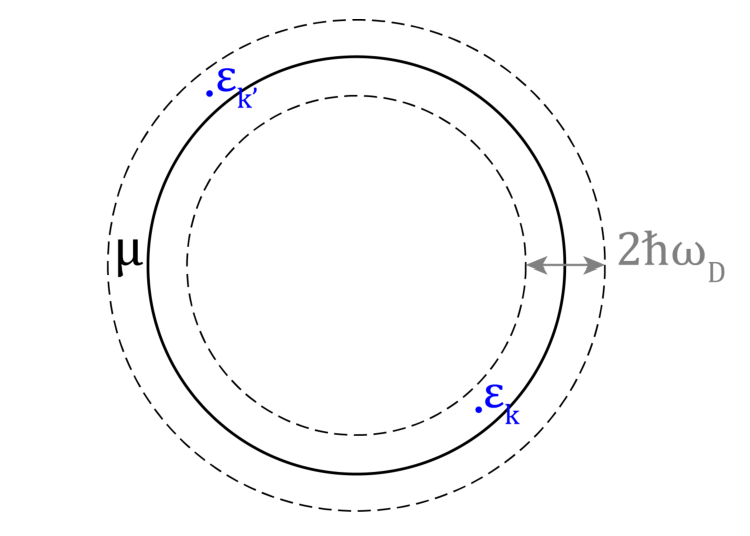
\includegraphics[width=0.8\textwidth]{img/2-bcs_energy_shell.png}
    \end{minipage}
    \hfill
    \begin{minipage}{0.45\textwidth}
        \caption{The model of the potential $V(\mathbf{k}', \mathbf{k})$ for superconductors is given by \eqref{eq:bcs_potential} and it involves just the fermions with energies $\epsilon_k$ and $\epsilon_{k'}$ residing strictly within a tiny energy shell of width $2\hbar\omega_D$ centered around the Fermi energy.}
        \label{fig:bcs_energy_shell}
    \end{minipage}
\end{figure}

To express this restricted interaction more compactly, it is highly advantageous to introduce a dimensionless cut-off function $w_k = \Theta(\hbar\omega_D - |\epsilon_k - \mu|)$, where $\Theta$ denotes the standard Heaviside step function. Utilizing this notation, the piecewise potential \eqref{eq:bcs_potential} can be elegantly rewritten in a strictly factorized form:
\begin{equation} \label{eq:bcs_potential_separable}
    V(\mathbf{k}', \mathbf{k}) = -g_{\text{e,ph}}^2 w_k w_{k'}.
\end{equation}
This mathematically represents the localized attractive potential acting exclusively between fermions scattered around the Fermi energy in a superconductor. Note that this specific theoretical form of the potential is entirely \emph{separable}; the dependence on the incoming momentum $\mathbf{k}$ and the outgoing momentum $\mathbf{k}'$ factors into independent terms, a property that will dramatically simplify the subsequent many-body calculations.

\subsection{Ultracold Fermi Gases}

As previously mentioned, the BCS theoretical framework can also be employed to study systems of ultracold Fermi atoms. In these highly controlled systems, the effective interparticle interaction possesses a very short range compared to the average interparticle distance. Because of this separation of scales, it is highly convenient to model the interaction using a separable potential in momentum space:
\[
    V(\mathbf{k}', \mathbf{k}) = v_0 w_k w_{k'},
\]
where $w_k = \Theta(k_0 - k)$ utilizes the Heaviside step function to introduce a strict \textit{ultraviolet momentum cutoff} $k_0$, and $v_0$ represents the bare interaction strength. Note that formally, this separable potential is structurally very similar to the one utilized for modeling electron-phonon interactions in superconductors.

\subsubsection{Scattering Theory}

For a genuinely short-range potential in position space, the corresponding cutoff in momentum space must be taken to be very large, meaning $k_0 \to \infty$. We thus need to understand how to appropriately treat this divergent limit mathematically. The core physical idea is that as the cutoff $k_0$ goes to infinity, the bare interaction parameter $v_0$ must simultaneously change with $k_0$ in a precise manner in order to keep the physically observable \textbf{scattering length} $a$ strictly constant.

To rigorously establish this relationship, we invoke the quantum theory of scattering.\footnote{For a comprehensive treatment, see, e.g., John R. Taylor, \textit{Scattering Theory: The Quantum Theory of Nonrelativistic Collisions} (Dover Books).} We know that the elastic scattering amplitude $f(\mathbf{k}', \mathbf{k}) \equiv f(\mathbf{k}' \leftarrow \mathbf{k})$ for scattering from an initial momentum $\mathbf{k}$ to a final momentum $\mathbf{k}'$ can be obtained directly from the T-matrix, $T(\mathbf{k}', \mathbf{k}, z)$. This T-matrix satisfies the fundamental \textit{Lippmann-Schwinger integral equation}:
\[
    T(\mathbf{k}', \mathbf{k}, z) = V(\mathbf{k}', \mathbf{k}) + \int \frac{\mathrm{d}^3 \mathbf{k}''}{(2\pi)^3} \frac{V(\mathbf{k}', \mathbf{k}'')}{z - \frac{(k'')^2}{2m_r}} T(\mathbf{k}'', \mathbf{k}, z),
\]
where $m_r$ is the reduced mass of the colliding two-body system, while $z$ is the complex energy variable. For a gas of identical fermions of mass $m$, the reduced mass is simply $m_r = m/2$. The formal relation linking the T-matrix to the physical scattering amplitude is evaluated on-shell:
\[
    f(\mathbf{k}', \mathbf{k}) = -\frac{m_r}{2\pi\hbar^2} T\left(\mathbf{k}', \mathbf{k}, z = \frac{\hbar^2k^2}{2m_r} + i0^+\right),
\]
where $i0^+$ is an infinitesimal positive imaginary term. In the extreme low-energy limit, the scattering amplitude limits to the negative of the scattering length, implying that:
\begin{equation} \label{eq:scattering_length_definition}
    T(0,0,0) = \frac{2\pi\hbar^2}{m_r} a.
\end{equation}
We can safely ignore the infinitesimal term $i0^+$ because it becomes entirely irrelevant for the principal value of the integral when evaluating at exactly $z = 0$. Here we are translating the physical requirement of a fixed scattering length $a$ into a precise mathematical condition on the bare interaction strength $v_0$ as a function of the ultraviolet cutoff $k_0$: it is a microscopic requirement that we have derived directly from mesoscopic scattering theory.

\subsubsection{Renormalization of the Bare Coupling Strength}

Because our proposed potential is purely separable and takes the form $V(\mathbf{k}', \mathbf{k}) = v_0 w_k w_{k'}$, the integral equation can be easily solved analytically. Substituting the potential yields:
\[
    T(\mathbf{k}', \mathbf{k}, z) = v_0 w_k w_{k'} + v_0 w_{k'} \int \frac{\mathrm{d}^3 \mathbf{k}''}{(2\pi)^3} \frac{w_{k''}}{z - \frac{(k'')^2}{2m_r}} T(\mathbf{k}'', \mathbf{k}, z).
\]
We can now employ the separable ansatz $T(\mathbf{k}', \mathbf{k}, z) = T(z) w_k w_{k'}$: we can do this since if we take \(\mathbf{k}\) and \(\mathbf{k}'\) to be out of the annulus defined by the cutoff, then \(T(\mathbf{k}', \mathbf{k}, z) = 0\) and the equation is trivially satisfied. Otherwise, if only one of \(\mathbf{k}\) or \(\mathbf{k}'\) is outside the annulus, then \(T(\mathbf{k}', \mathbf{k}, z) = 0\) because it has to be invariant under the exchange of \(\mathbf{k}\) and \(\mathbf{k}'\). Thus, we factor out the momentum dependence and obtain a simple algebraic equation for the scalar function $T(z)$:\TODO{explain better the ansatz}
\[
    T(z) = v_0 + v_0 \int \frac{\mathrm{d}^3 \mathbf{k}''}{(2\pi)^3} \frac{w_{k''}^2}{z - \frac{(k'')^2}{2m_r}} T(z).
\]
This equation is readily solved for $T(z)$, yielding:
\[
    T(z) = \frac{v_0}{1 - v_0 \int \frac{\mathrm{d}^3 \mathbf{k}''}{(2\pi)^3} \frac{w_{k''}^2}{z - \frac{(k'')^2}{2m_r}}}.
\]
Setting $z=0$ to connect with our low-energy scattering length boundary condition provides:
\[
    T(0) = \frac{1}{\frac{1}{v_0} + \int \frac{\mathrm{d}^3 \mathbf{k}}{(2\pi)^3} \frac{w_k^2}{\frac{k^2}{2m_r}}}.
\]
Equating this result to the previously derived kinematic definition for the scattering length, $T(0,0,0) = \frac{4\pi\hbar^2}{m} a$ (where we have substituted $m_r = m/2$ w.r.t. \eqref{eq:scattering_length_definition}), we obtain:
\[
    \frac{4\pi\hbar^2}{m} a = \frac{1}{\frac{1}{v_0} + \int \frac{\mathrm{d}^3 \mathbf{k}}{(2\pi)^3} \frac{w_k^2}{\frac{k^2}{2m_r}}}.
\]

\begin{remark}
    Since we used \eqref{eq:scattering_length_definition} to define the scattering length, this relation is valid in the low-energy limit, where the scattering amplitude is independent of the incoming and outgoing momenta. In this limit, the scattering length is a universal quantity that characterizes the low-energy scattering properties of the system, independent of the specific details of the interaction potential.
\end{remark}

By isolating the inverse bare coupling strength, we can rewrite this relation as:
\begin{equation} \label{eq:bare_coupling_renormalization}
    \frac{1}{v_0} = \frac{m}{4\pi\hbar^2 a} - \int \frac{\mathrm{d}^3 \mathbf{k}}{(2\pi)^3} \frac{w_k^2}{2\epsilon_k},
\end{equation}
where we have explicitly used the free-particle kinetic energy dispersion $\epsilon_k = \hbar^2 k^2 / 2m$. Equation \eqref{eq:bare_coupling_renormalization} reveals how the bare interaction strength $v_0$ must scale intricately with the ultraviolet momentum cutoff $k_0$ (which is embedded within the definition of $w_k$) when the macroscopic scattering length $a$ is held strictly fixed. This mathematical behavior is deeply analogous to a \textit{running coupling constant} in quantum field theory. It is critical to note that \eqref{eq:bare_coupling_renormalization} \uline{is universally valid for any generic separable potential, independent of the specific functional form chosen for the cutoff $w_k$}.

For our specific hard-sphere cutoff model, $w_k = \Theta(k_0 - k)$, the integral can be evaluated analytically in spherical coordinates, yielding:
\[
    v_0 = \frac{\hbar^2}{m} \frac{1}{\frac{1}{4\pi a} - \frac{k_0}{2\pi^2}}.
\]
To analyze the physics of a true zero-range contact interaction, we take the limit as the cutoff $k_0 \to \infty$ while holding $a$ constant (such that the dimensionless parameter $k_0 a \gg 1$). Expanding the expression in this limit gives:
\[
    v_0 = -\frac{2\pi^2\hbar^2}{m k_0} \left[ 1 + \frac{\pi}{2k_0 a} \right].
\]
This asymptotic expansion clearly demonstrates that in the limiting case of a perfectly localized contact potential, the bare coupling strength must approach zero from below, $v_0 \to 0^-$, as $k_0 \to \infty$. Notice also that the physical scattering length $a$ appears exclusively in the subleading term on the right-hand side of this limiting expression. Finally, we are not really concerned with the fact of having a momentum cutoff in the interaction, since the physical scattering length is a well-defined quantity that can be measured experimentally and we are not really interested in the microscopic details of the interaction potential, expecially at such high momenta.

\section{Grand Canonical Hamiltonian and Ground State}

Let us now proceed to study the many-body problem. We will work within the grand canonical ensemble, where the thermodynamic properties of the system are governed by the partition function \( \mathcal{Z} \), defined as:
\[
    \mathcal{Z} = \text{Tr}\left\{e^{-\beta \hat{K}}\right\},
\]
where \( \hat{K} = \hat{H} - \mu \hat{N} \) is the grand canonical ``Hamiltonian'', \( \mu \) is the chemical potential, and \( \hat{N} \) is the fermionic number operator.

Notice that \uline{the partition function \( \mathcal{Z} \) is not an observable}: it is a purely mathematical object that encodes the statistical properties of the system, which is related to different microscopic and thermodinamic observables; but it is also a matrix with a number of eigenvalues that grows exponentially with the number of particles in the system: this makes it impossible to compute exactly for a many-body system.

Using the standard second-quantized expression for the interaction, \( \hat{K} \) takes the form:
\[
    \hat{K} = \sum_{\mathbf{k},\sigma} \xi_k c_{\mathbf{k},\sigma}^\dagger c_{\mathbf{k},\sigma} + \frac{1}{2V} \sum_{\mathbf{k},\mathbf{k}',\mathbf{q}} \sum_{\sigma,\sigma'} V(\mathbf{k}', \mathbf{k}) c_{\mathbf{k}'+\frac{\mathbf{q}}{2},\sigma}^\dagger c_{-\mathbf{k}'+\frac{\mathbf{q}}{2},\sigma'}^\dagger c_{-\mathbf{k}+\frac{\mathbf{q}}{2},\sigma'} c_{\mathbf{k}+\frac{\mathbf{q}}{2},\sigma},
\]
where we have defined the single-particle kinetic energy relative to the chemical potential as \( \xi_k = \epsilon_k - \mu \).\footnote{This follows straightforwardly from the definition of the grand canonical Hamiltonian.} For notational convenience, we will write the non-interacting kinetic part of \( \hat{K} \) as \( \hat{T} \).

We are fundamentally interested in the pairing mechanism between fermions of opposite spin (spin up \( \uparrow \) and spin down \( \downarrow \)), as this is the dominant process in most conventional superconductors. The interaction between identical fermions (same spin) is irrelevant for the pairing mechanism and can thus be safely ignored, since it exerts only a negligible effect on the physical properties of a superconductor. Furthermore, in the specific case of ultracold Fermi gases, the effective interaction is strictly short-ranged, meaning only interactions between up and down fermions need to be considered; the presence of two identical fermions in the same spatial region is strongly suppressed by the Pauli exclusion principle. By restricting the interaction term to couple only opposite spins, and performing the summation over the spin indices \( \sigma \) and \( \sigma' \), we obtain:
\[
    \hat{K} = \hat{T} + \frac{1}{V} \sum_{\mathbf{k},\mathbf{k}',\mathbf{q}} V(\mathbf{k}', \mathbf{k}) c_{\mathbf{k}'+\frac{\mathbf{q}}{2},\uparrow}^\dagger c_{-\mathbf{k}'+\frac{\mathbf{q}}{2},\downarrow}^\dagger c_{-\mathbf{k}+\frac{\mathbf{q}}{2},\downarrow} c_{\mathbf{k}+\frac{\mathbf{q}}{2},\uparrow}.
\]

Keep in mind that all these summations are considering only momenta within a narrow shell around the Fermi surface, for which the effective interaction is non-zero.

Furthermore this hamiltonian has an \(U(1)\) symmetry, which is the symmetry associated with the conservation of the number of particles: it commutes with the number operator \(\hat{N}\) and there are no terms that create or destroy particles without compensating for it. Furthermore we have a spin-symmetry (called also asymmetric charge) goven by the difference between the number of spin-up and spin-down particles, which is also conserved. This symmetry is associated with the conservation of the total spin of the system, since for any spin-up particle that is created, a spin-down particle is also created, and vice versa (or a spin-up particle isdestroyed).

\subsection{Mean-Field Approximation}

We now proceed in a manner conceptually similar to the treatment of the weakly-interacting Bose gas, with the primary difference being that in the present fermionic case, we anticipate the macroscopic condensation of \emph{pairs} of fermions rather than individual particles.\footnote{Since fermionic wavefunctions are antisymmetric, when we compute expectation values of fermionic operators we are taking a tensor product of something foundamentally antisymmetric (\(c \ket{\psi_{GS}}\)) and something foundamentally symmetric (\(\bra{\psi_{GS}}\)): this makes the computation of expectation values more complex. We cannot take the expectation value of fermionic operators directly.} Consider the pair destruction operator factor \( c_{-\mathbf{k}+\frac{\mathbf{q}}{2},\downarrow} c_{\mathbf{k}+\frac{\mathbf{q}}{2},\uparrow} \) embedded in the interaction term, which will give rise to an interaction term between \textbf{Cooper pairs}. We rewrite it (keeping all momentum and spin indices implicit for brevity) by expanding around its thermodynamic mean:
\[
    cc = cc - \langle cc \rangle + \langle cc \rangle = \delta(cc) + \langle cc \rangle,
\]
where \( \delta(cc) = cc - \langle cc \rangle \) represents the deviation (or fluctuation) of the operator \( cc \) from its expectation value \( \langle cc \rangle \). We will assume this deviation to be a small quantity and apply the exact same decomposition to the pair creation factor \( c^\dagger c^\dagger \). Substituting these back into the interaction and systematically neglecting the second-order fluctuation term of order \( \delta(c^\dagger c^\dagger)\delta(cc) \), the four-operator interaction is linearized into a bilinear form:
\[
    \begin{aligned}
        c^\dagger c^\dagger cc & = \delta(c^\dagger c^\dagger) \langle cc \rangle + \langle c^\dagger c^\dagger \rangle \delta(cc) + \langle c^\dagger c^\dagger \rangle \langle cc \rangle \\
                               & = c^\dagger c^\dagger \langle cc \rangle + \langle c^\dagger c^\dagger \rangle cc - \langle c^\dagger c^\dagger \rangle \langle cc \rangle.
    \end{aligned}
\]

We have already made an argument to exploit the anti-alignement of the spins of the two fermions in a Cooper pair, which is a fundamental property of the BCS theory. This allows us to restrict our attention to the spin-up and spin-down components of the fermionic operators, as we have done in the above expressions. But we have to still take into account the momentum of the pairs, which is represented by the center-of-mass momentum \( \mathbf{q} \). Because the macroscopic condensation of pairs is physically expected to occur exactly at zero center-of-mass momentum, the expectation values are non-zero only for \( \mathbf{q} = 0 \). Thus, we can rigorously set: \TODO{add figure of opposing momentum fermions in the annulus as only allowed to interact to form a Cooper pair with zero center-of-mass momentum}
\[
    \begin{aligned}
        \langle c_{-\mathbf{k}+\frac{\mathbf{q}}{2},\downarrow} c_{\mathbf{k}+\frac{\mathbf{q}}{2},\uparrow} \rangle                   & = \delta_{\mathbf{q},0} A_{\mathbf{k}}\, ,    \\
        \langle c_{\mathbf{k}'+\frac{\mathbf{q}}{2},\uparrow}^\dagger c_{-\mathbf{k}'+\frac{\mathbf{q}}{2},\downarrow}^\dagger \rangle & = \delta_{\mathbf{q},0} A_{\mathbf{k}'}^*\, ,
    \end{aligned}
\]
where \( A_{\mathbf{k}} \) is a function of the momentum \( \mathbf{k} \) that remains to be determined. Substituting this mean-field ansatz, the grand canonical Hamiltonian simplifies to:
\[
    \hat{K} = \hat{T} + \frac{1}{V} \sum_{\mathbf{k},\mathbf{k}'} V(\mathbf{k}', \mathbf{k}) \left[ c_{\mathbf{k}',\uparrow}^\dagger c_{-\mathbf{k}',\downarrow}^\dagger A_{\mathbf{k}} + c_{-\mathbf{k},\downarrow} c_{\mathbf{k},\uparrow} A_{\mathbf{k}'}^* \right] - \frac{1}{V} \sum_{\mathbf{k},\mathbf{k}'} V(\mathbf{k}', \mathbf{k}) A_{\mathbf{k}'}^* A_{\mathbf{k}}.
\]

To render this expression more physically transparent, we define the \textit{momentum-dependent superconducting} \textbf{gap parameter} \( \Delta_{\mathbf{k}} \) and its complex conjugate:
\begin{equation} \label{eq:gap_definition}
    \Delta_{\mathbf{k}'} = - \frac{1}{V} \sum_{\mathbf{k}} V(\mathbf{k}', \mathbf{k}) A_{\mathbf{k}}, \quad \Delta_{\mathbf{k}}^* = - \frac{1}{V} \sum_{\mathbf{k}'} V(\mathbf{k}', \mathbf{k}) A_{\mathbf{k}'}^*.
\end{equation}
Note that these definitions are perfectly consistent because any time-reversal invariant potential satisfies the symmetry \( V(\mathbf{k}, \mathbf{k}') = V(\mathbf{k}', \mathbf{k})^* \). With these definitions, one obtains a bilinear Hamiltonian:
\[
    \hat{K} = \hat{T} - \sum_{\mathbf{k}} \left[ \Delta_{\mathbf{k}} c_{\mathbf{k},\uparrow}^\dagger c_{-\mathbf{k},\downarrow}^\dagger + \Delta_{\mathbf{k}}^* c_{-\mathbf{k},\downarrow} c_{\mathbf{k},\uparrow} \right] + \sum_{\mathbf{k}} A_{\mathbf{k}}^* \Delta_{\mathbf{k}}.
\]
Notice that the last term is a constant energy offset that does not depend on the fermionic operators. Usually one discards such terms, but in this case it is important to keep it because it is a function of the gap parameter \( \Delta_{\mathbf{k}} \) and thus it will contribute to the self-consistent equation for the gap. We will assume anyway that the Ground State solution will be independent of such constant term, and we will see that this is indeed the case.

The Gaussian Problem we have obtained is a quadratic Hamiltonian in the fermionic operators, which can be solved exactly. The only unknowns are the gap parameters \( \Delta_{\mathbf{k}} \) and \( \Delta_{\mathbf{k}}^* \), which will be determined self-consistently by solving the gap equation \eqref{eq:gap_definition}.

\subsection{Diagonalization of the Hamiltonian}

To elegantly diagonalize this bilinear Hamiltonian, it is highly convenient to express it in a matrix representation using \textbf{Nambu spinors}. By leveraging the fundamental fermionic anti-commutation relations, we can rewrite the kinetic energy term for the spin-down particles as
\[
    \xi_k c_{\mathbf{k},\downarrow}^\dagger c_{\mathbf{k},\downarrow} = \xi_k - \xi_k c_{\mathbf{k},\downarrow} c_{\mathbf{k},\downarrow}^\dagger \, .
\]
Now we notice that in the Hamiltonian we have terms proportional to \(cc, cc^\dagger, c^\dagger c, c^\dagger c^\dagger\), and such combinations can be expressed in terms of matrices of the form\TODO{put momentum and spin pedices}
\[
    \begin{pmatrix}
        c^{\dagger} c & c^{\dagger}  c^\dagger \\
        c c           & c c^\dagger
    \end{pmatrix}\, .
\]
This algebraic maneuver allows us to recast the operator \( \hat{K} \) into the following compact matrix form:
\begin{equation} \label{eq:nambu_hamiltonian}
    \hat{K} = \sum_{\mathbf{k}} \begin{pmatrix} c_{\mathbf{k},\uparrow}^\dagger & c_{-\mathbf{k},\downarrow} \end{pmatrix} \begin{pmatrix} \xi_k & -\Delta_{\mathbf{k}} \\ -\Delta_{\mathbf{k}}^* & -\xi_k \end{pmatrix} \begin{pmatrix} c_{\mathbf{k},\uparrow} \\ c_{-\mathbf{k},\downarrow}^\dagger \end{pmatrix} + C,
\end{equation}
where the constant energy offset \( C \) is explicitly given by all the terms which do not depend on the fermionic operators:
\[
    C = \sum_{\mathbf{k}} \left( \xi_k + A_{\mathbf{k}}^* \Delta_{\mathbf{k}} \right).
\]
Notice that the off-diagonal terms in the matrix representation of \( \hat{K} \) are proportional to the gap parameter \( \Delta_{\mathbf{k}} \), which lets operators of opposite momenta couple to each other. This is a direct manifestation of the fundamental pairing mechanism that underlies the BCS theory of superconductivity. The constant term is important, but we want to ``solve the problem'' (diagonalize the Hamiltonian) in order to find the ground state and the quasiparticle excitations, without having to worry about the constant term, which will be added at the end.

\subsubsection{Quasiparticle Transformation}

Let us define the central \( 2 \times 2 \) Hermitian matrix \( M_{\mathbf{k}} \) as:
\[
    M_{\mathbf{k}} = \begin{pmatrix} \xi_k & -\Delta_{\mathbf{k}} \\ -\Delta_{\mathbf{k}}^* & -\xi_k \end{pmatrix}.
\]

We now show that the many-body problem of diagonalizing the quadratic form \( \hat{K} \) reduces entirely to the problem of diagonalizing the independent \( 2 \times 2 \) matrix \( M_{\mathbf{k}} \) for every momentum mode \( \mathbf{k} \). In strict analogy to the procedure utilized for the weakly interacting Bose gas (with the Bogoliubov transformation and quasiparticles), we seek a transformation to a new set of fermionic creation and destruction operators, \( \gamma_{\mathbf{k},\sigma} \) and \( \gamma_{\mathbf{k},\sigma}^\dagger \), that diagonalize \( \hat{K} \). These will become our new \textit{quasiparticle operators}. We introduce a transformation matrix \( U_{\mathbf{k}} \) such that:
\begin{equation} \label{eq:bogoliubov_transform}
    \begin{pmatrix} c_{\mathbf{k},\uparrow} \\ c_{-\mathbf{k},\downarrow}^\dagger \end{pmatrix} = U_{\mathbf{k}} \begin{pmatrix} \gamma_{\mathbf{k},\uparrow} \\ \gamma_{-\mathbf{k},\downarrow}^\dagger \end{pmatrix}, \quad \begin{pmatrix} c_{\mathbf{k},\uparrow}^\dagger & c_{-\mathbf{k},\downarrow} \end{pmatrix} = \begin{pmatrix} \gamma_{\mathbf{k},\uparrow}^\dagger & \gamma_{-\mathbf{k},\downarrow} \end{pmatrix} U_{\mathbf{k}}^\dagger.
\end{equation}
Notice that we are mixing momenta and spins in this transformation, which is a direct consequence of the fundamental pairing mechanism that underlies the BCS theory (the structure of the Hamiltonian encodes this directly).

This transformation must simultaneously satisfy two critical conditions:
\begin{enumerate}
    \item The terms appearing in the grand canonical Hamiltonian, once expressed in terms of the new operators, must form a diagonal matrix \( D_{\mathbf{k}} \):
          \[
              \begin{pmatrix} c_{\mathbf{k},\uparrow}^\dagger & c_{-\mathbf{k},\downarrow} \end{pmatrix} M_{\mathbf{k}} \begin{pmatrix} c_{\mathbf{k},\uparrow} \\ c_{-\mathbf{k},\downarrow}^\dagger \end{pmatrix} = \begin{pmatrix} \gamma_{\mathbf{k},\uparrow}^\dagger & \gamma_{-\mathbf{k},\downarrow} \end{pmatrix} U_{\mathbf{k}}^\dagger M_{\mathbf{k}} U_{\mathbf{k}} \begin{pmatrix} \gamma_{\mathbf{k},\uparrow} \\ \gamma_{-\mathbf{k},\downarrow}^\dagger \end{pmatrix},
          \]
          with \( D_{\mathbf{k}} = U_{\mathbf{k}}^\dagger M_{\mathbf{k}} U_{\mathbf{k}} \) being explicitly diagonal: \(U_{\mathbf{k}}\) is a unitary (as we will see in a moment) change of basis that diagonalizes the Hamiltonian.
    \item The fundamental anti-commutation rules must be preserved for the new quasiparticle operators, ensuring in particular that:
          \[
              \{ \gamma_{\mathbf{k},\sigma}, \gamma_{\mathbf{k}',\sigma'}^\dagger \} = \delta_{\mathbf{k},\mathbf{k}'} \delta_{\sigma,\sigma'},
          \]
          with all remaining anti-commutators identically zero.
\end{enumerate}

We can readily prove that \uline{requiring the transformation \( U_{\mathbf{k}} \) to be unitary guarantees the preservation of these anti-commutation relations} on the new operators.
\begin{proof}
    Let us parameterize the inverse transformation matrix as:
    \[
        U_{\mathbf{k}}^{-1} = \begin{pmatrix} a_{11} & a_{12} \\ a_{21} & a_{22} \end{pmatrix}.
    \]
    The relation linking the bare \( c \) operators to the quasiparticle \( \gamma \) operators is then:
    \[
        \begin{pmatrix} \gamma_{\mathbf{k},\uparrow} \\ \gamma_{-\mathbf{k},\downarrow}^\dagger \end{pmatrix} = U_{\mathbf{k}}^{-1} \begin{pmatrix} c_{\mathbf{k},\uparrow} \\ c_{-\mathbf{k},\downarrow}^\dagger \end{pmatrix}, \quad \begin{pmatrix} \gamma_{\mathbf{k},\uparrow}^\dagger & \gamma_{-\mathbf{k},\downarrow} \end{pmatrix} = \begin{pmatrix} c_{\mathbf{k},\uparrow}^\dagger & c_{-\mathbf{k},\downarrow} \end{pmatrix} (U_{\mathbf{k}}^{-1})^\dagger,
    \]
    where \((U_{\mathbf{k}}^{-1})^\dagger\) is the conjugate transpose of \(U_{\mathbf{k}}^{-1}\):
    \[
        (U_{\mathbf{k}}^{-1})^\dagger = \begin{pmatrix} a_{11}^* & a_{21}^* \\ a_{12}^* & a_{22}^* \end{pmatrix}.
    \]
    By explicitly substituting this into the anti-commutators and using the known algebraic relations for the bare \( c \) operators, it is straightforward to check that:\TODO{check computations from Di Sante notes (Filippo)}
    \[
        \{ \gamma_{\mathbf{k},\uparrow}, \gamma_{\mathbf{k}',\uparrow}^\dagger \} = \left\{ \left(a_{11} c_{\mathbf{k},\uparrow} + a_{12} c_{-\mathbf{k},\downarrow}^\dagger\right), \left(a_{11}^* c_{\mathbf{k}',\uparrow}^* + a_{12}^* c_{-\mathbf{k}',\downarrow}^\dagger\right) \right\}= (|a_{11}|^2 + |a_{12}|^2) \delta_{\mathbf{k},\mathbf{k}'},
    \]
    \[
        \{ \gamma_{-\mathbf{k},\downarrow}, \gamma_{-\mathbf{k}',\downarrow}^\dagger \} = \left\{ \left(a_{21} c_{-\mathbf{k},\downarrow} + a_{22} c_{\mathbf{k},\uparrow}^\dagger\right), \left(a_{21}^* c_{-\mathbf{k}',\downarrow}^* + a_{22}^* c_{\mathbf{k}',\uparrow}^*\right) \right\} = (|a_{21}|^2 + |a_{22}|^2) \delta_{\mathbf{k},\mathbf{k}'},
    \]
    \[
        \{ \gamma_{\mathbf{k},\uparrow}, \gamma_{-\mathbf{k}',\downarrow} \} = \left\{ \left(a_{11} c_{\mathbf{k},\uparrow} + a_{12} c_{-\mathbf{k},\downarrow}^\dagger\right), \left(a_{21}^* c_{-\mathbf{k}',\downarrow}^* + a_{22}^* c_{\mathbf{k}',\uparrow}^*\right) \right\} = (a_{11} a_{21}^* + a_{12} a_{22}^*) \delta_{\mathbf{k},-\mathbf{k}'}.
    \]
    In order to successfully satisfy the fermionic algebra, the coefficients must obey:
    \[
        1 = |a_{11}|^2 + |a_{12}|^2,
    \]
    \[
        1 = |a_{21}|^2 + |a_{22}|^2,
    \]
    \[
        0 = a_{11} a_{21}^* + a_{12} a_{22}^*.
    \]
    These three constraints are automatically and exactly satisfied by unitary matrices. This implies that \( U_{\mathbf{k}}^\dagger M_{\mathbf{k}} U_{\mathbf{k}} = U_{\mathbf{k}}^{-1} M_{\mathbf{k}} U_{\mathbf{k}} \); thus, finding a unitary matrix that diagonalizes the Hermitian matrix \( M_{\mathbf{k}} \) will successfully diagonalize the entire many-body Hamiltonian \( \hat{K} \).
\end{proof}

\subsubsection{Quasiparticle Dispersion and Coherence Factors}

The eigenvalues \( \lambda \) of \( M_{\mathbf{k}} \) are determined by its characteristic equation:
\[
    (\xi_k - \lambda)(-\xi_k - \lambda) - |\Delta_{\mathbf{k}}|^2 = 0,
\]
from which we immediately obtain the roots \( \lambda = \pm E_{\mathbf{k}} \), where:
\begin{equation} \label{eq:quasiparticle_dispersion}
    E_{\mathbf{k}} = \sqrt{\xi_k^2 + |\Delta_{\mathbf{k}}|^2} > 0.
\end{equation}
This fundamentally important quantity \( E_{\mathbf{k}} \) represents the \textit{energy dispersion of the superconducting quasiparticle excitations}. We expected two opposite sign eigenvalues because the Hamiltonian ...

If we let the gap parameter \( \Delta_{\mathbf{k}} \) vanish, the quasiparticle dispersion reduces to the free-particle kinetic energy relative to the chemical potential, \( E_{\mathbf{k}} = |\xi_k| \). In this limit, the quasiparticles are simply the original bare fermions.

The normalized eigenvector of \( M_{\mathbf{k}} \) corresponding to the positive eigenvalue \( E_{\mathbf{k}} \) takes the form:
\[
    \begin{pmatrix} u_{\mathbf{k}}^* \\ -v_{\mathbf{k}}^* \end{pmatrix}, \text{ with } \vert u_{\mathbf{k}} \vert^2 + \vert v_{\mathbf{k}} \vert^2 = 1.
\]
Following this definition, the \textbf{coherence factors} can be expressed as:
\[
    u_{\mathbf{k}}^* = \frac{\Delta_{\mathbf{k}}}{\sqrt{2E_{\mathbf{k}}(E_{\mathbf{k}} - \xi_k)}}, \quad v_{\mathbf{k}}^* = \frac{E_{\mathbf{k}} - \xi_k}{\sqrt{2E_{\mathbf{k}}(E_{\mathbf{k}} - \xi_k)}} = v_{\mathbf{k}},
\]
such that \(v_{\mathbf{k}} \) will be strictly real and positive, while \(u_{\mathbf{k}}\) can be complex.

Conversely, the normalized eigenvector corresponding to the negative eigenvalue \( -E_{\mathbf{k}} \) is:
\[
    \begin{pmatrix} v_{\mathbf{k}} \\ u_{\mathbf{k}} \end{pmatrix}.
\]
\begin{remark}
    In defining these eigenvectors, a specific choice of phase factors has been made such that \( v_{\mathbf{k}}^* \) is strictly real and the determinant of the transformation matrix is exactly \( \det U_{\mathbf{k}} = 1 \).
\end{remark}
Using these two orthogonal eigenvectors, one may immediately construct the explicit unitary transformation \( U_{\mathbf{k}} \) that diagonalizes \( M_{\mathbf{k}} \):
\[
    U_{\mathbf{k}} = \begin{pmatrix} u_{\mathbf{k}}^* & v_{\mathbf{k}} \\ -v_{\mathbf{k}}^* & u_{\mathbf{k}} \end{pmatrix},
\]
with its corresponding inverse:
\[
    U_{\mathbf{k}}^{-1} = U_{\mathbf{k}}^\dagger = \begin{pmatrix} u_{\mathbf{k}} & -v_{\mathbf{k}} \\ v_{\mathbf{k}}^* & u_{\mathbf{k}}^* \end{pmatrix}.
\]

\subsubsection{Bogoliubov Transformation and Diagonalized Hamiltonian}

By applying the previously derived inverse transformation, we obtain the explicit mathematical expressions for the new operators in terms of the old ones (the celebrated Bogoliubov transformation):
\begin{equation} \label{eq:bogoliubov_operators}
    \gamma_{\mathbf{k},\uparrow} = u_{\mathbf{k}} c_{\mathbf{k},\uparrow} - v_{\mathbf{k}} c_{-\mathbf{k},\downarrow}^\dagger,
\end{equation}
\[
    \gamma_{-\mathbf{k},\downarrow}^\dagger = v_{\mathbf{k}}^* c_{\mathbf{k},\uparrow} + u_{\mathbf{k}}^* c_{-\mathbf{k},\downarrow}^\dagger.
\]
Notice that the new annihilation operator \( \gamma_{\mathbf{k},\uparrow} \) physically mixes the old creation operator \( c_{-\mathbf{k},\downarrow}^\dagger \) and destruction operator \( c_{\mathbf{k},\uparrow} \), specifically entangling particles with opposite spin and momentum.\footnote{Equivalently, taking the Hermitian adjoint of the second equation yields \( \gamma_{-\mathbf{k},\downarrow} = u_{\mathbf{k}} c_{-\mathbf{k},\downarrow} + v_{\mathbf{k}} c_{\mathbf{k},\uparrow}^\dagger \).}

In these transformed variables, spin plays a non trivial role, as the same operator creates a particle with spin up and destroys a particle with spin down. This is a direct consequence of the pairing mechanism, which couples opposite spins and momenta, preserving the \textit{parity symmetry} \(\mathrm{Z}_2\) of the system. The Bogoliubov transformation is a canonical unitary transformation that preserves the fundamental anti-commutation relations.

Thinking about the \textit{Stern-Gerlach experiment}, we can see that the new quasiparticle operators \( \gamma_{\mathbf{k},\sigma} \) and \( \gamma_{\mathbf{k},\sigma}^\dagger \) do not correspond to any physical spin measurement along a given axis. Instead, they represent a superposition of spin-up and spin-down states, which is a direct manifestation of the entanglement between opposite spins induced by the pairing mechanism of BCS theory.

Expressed in terms of these newly defined \( \gamma \) operators, the grand canonical Hamiltonian assumes its fully diagonalized form:
\[
    \hat{K} = \sum_{\mathbf{k}} \begin{pmatrix} \gamma_{\mathbf{k},\uparrow}^\dagger & \gamma_{-\mathbf{k},\downarrow} \end{pmatrix} D_{\mathbf{k}} \begin{pmatrix} \gamma_{\mathbf{k},\uparrow} \\ \gamma_{-\mathbf{k},\downarrow}^\dagger \end{pmatrix} + C,
\]
where the diagonal eigenvalue matrix \( D_{\mathbf{k}} = U_{\mathbf{k}}^\dagger M_{\mathbf{k}} U_{\mathbf{k}} \) is given by:
\[
    D_{\mathbf{k}} = \begin{pmatrix} E_{\mathbf{k}} & 0 \\ 0 & -E_{\mathbf{k}} \end{pmatrix}.
\]
By explicitly expanding this matrix product and once again applying the quasiparticle anti-commutation relations, we obtain:
\begin{equation} \label{eq:diagonalized_canonical_hamiltonian}
    \hat{K} = \sum_{\mathbf{k}} \left( E_{\mathbf{k}} \gamma_{\mathbf{k},\uparrow}^\dagger \gamma_{\mathbf{k},\uparrow} - E_{\mathbf{k}} \gamma_{-\mathbf{k},\downarrow} \gamma_{-\mathbf{k},\downarrow}^\dagger \right) + C = \sum_{\mathbf{k},\sigma} E_{\mathbf{k}} \gamma_{\mathbf{k},\sigma}^\dagger \gamma_{\mathbf{k},\sigma} + C',
\end{equation}
where the newly defined constant term \( C' \) absorbs the commutation shifts, assuring that the Hamiltonian is expressed in normal-ordered form:
\[
    C' = C - \sum_{\mathbf{k}} E_{\mathbf{k}} = \sum_{\mathbf{k}} \left( \xi_k + A_{\mathbf{k}}^* \Delta_{\mathbf{k}} - E_{\mathbf{k}} \right).
\]
Because the quasiparticle energy dispersion \( E_{\mathbf{k}} \) is strictly positive, the operator \( \sum_{\mathbf{k},\sigma} E_{\mathbf{k}} \gamma_{\mathbf{k},\sigma}^\dagger \gamma_{\mathbf{k},\sigma} \) is positive semi-definite. Consequently, the constant \( C' \) physically represents the lowest possible eigenvalue of \( \hat{K} \), which corresponds exactly to the ground state grand potential of the superconducting system.

\subsection{Ground State Wave Function}

The structure of the many-body wavefunction will change dramatically in the superconducting phase, considering also that the occupation of the quasiparticle states is now governed by the Fermi-Dirac distribution. But the ground state of the system is still defined as the state with the lowest possible energy, and can be easily obtained.

In the grand-canonical ensemble, the thermodynamic thermal average of any physical operator \( \hat{O} \) is given by the standard statistical mechanics trace formula:
\[
    \langle O \rangle = \frac{\text{tr}\left(e^{-\beta \hat{K}} \hat{O}\right)}{\mathcal{Z}},
\]
where the grand partition function is defined as:
\[
    \mathcal{Z} = \text{tr}\left(e^{-\beta \hat{K}}\right).
\]
Here, \( \hat{K} = \hat{H} - \mu \hat{N} \) represents the grand canonical Hamiltonian. In the absolute zero temperature limit, \( T \to 0 \), the inverse temperature \( \beta \to +\infty \). In this asymptotic regime, the thermal average strictly reduces to a pure quantum mechanical expectation value over the ground state, where the grand-canonical ground state \( |\psi_0(\mu)\rangle \) is defined as the eigenstate of \( \hat{K} \) corresponding to its lowest possible eigenvalue\footnote{We are assuming that the ground state is unique. If this is not the case, a sum over all degenerate ground states would be required to evaluate the expectation values properly.}.

Based on our preceding diagonalization procedure, the lowest energy state corresponds to the configuration devoid of any quasiparticle excitations (since the quasiparticle energy is strictly positive). Therefore, in the present case, \( |\psi_0(\mu)\rangle \) is precisely the vacuum of the new Bogoliubov operators \( \gamma_{\mathbf{k},\sigma} \), meaning that it must satisfy the annihilation condition:
\begin{equation} \label{eq:bcs_vacuum_condition_gamma}
    \gamma_{\mathbf{k},\sigma} |\psi_0\rangle = 0 \quad \forall \mathbf{k}, \sigma.
\end{equation}
By explicitly using the Bogoliubov transformation derived earlier to express \( \gamma_{\mathbf{k},\uparrow} \) in terms of the bare particle operators,\footnote{For the sake of finding measurable observables, since the quasiparticles are a mathematical construct: we need correlation functions of the old fermionic variables, which can be measured.} this vacuum condition for the specific spin-up branch (\( \sigma = \uparrow \)) yields:
\begin{equation} \label{eq:bcs_vacuum_condition_bare}
    u_{\mathbf{k}} c_{\mathbf{k},\uparrow} |\psi_0\rangle = v_{\mathbf{k}} c_{-\mathbf{k},\downarrow}^\dagger |\psi_0\rangle.
\end{equation}

Looking at \eqref{eq:bcs_vacuum_condition_bare}, we can observe a profound physical symmetry: \uline{the action of destroying a bare fermion with momentum \( \mathbf{k} \) and spin \( \uparrow \) on the ground state is directly proportional to creating a bare fermion with opposite momentum \( -\mathbf{k} \) and opposite spin \( \downarrow \)}. This is a direct manifestation of Spontaneous Symmetry Breaking of the \( U(1) \) symmetry (conservation of particle number, broken in the ground state)
\[
    N_{\uparrow} + N_{\downarrow} broken
\]
\[
    N_{\uparrow} - N_{\downarrow} conserved
\]
commutator with hamiltonian...

U(1) charge and U(1) spin symmetries are preserved, but the U(1) particle number symmetry is spontaneously broken in the superconducting phase... it is not a gauge symmetry: gauge symmetries cannot be broken, there is a theorem.

The gamma operators are a linear combination of the bare fermionic operators, and they do not commute with the parity operator \( P = \prod_{\mathbf{k}, \sigma} (1-2n_{\mathbf{k},\sigma})\). But they preserve parity as a good quantum number, because they always create or destroy pairs of fermions. Indeed we have:\TODO{check computation (erio)}
\[
    \begin{aligned}
        \gamma_{\mathbf{k}, \uparrow} \ket{\psi} & = \left( u_{\mathbf{k}} c_{\mathbf{k},\uparrow} - v_{\mathbf{k}} c_{-\mathbf{k},\downarrow}^\dagger \right) (c_{\mathbf{k},\uparrow}^\dagger + c_{\mathbf{p},\downarrow}^\dagger) \ket{0} \\
                                                 & = u_{\mathbf{k}} c_{\mathbf{k},\uparrow} c_{\mathbf{k},\uparrow}^\dagger \ket{0} - v_{\mathbf{k}} c_{-\mathbf{k},\downarrow}^\dagger c_{\mathbf{p},\downarrow}^\dagger \ket{0}            \\
                                                 & = u_{\mathbf{k}} \ket{0} - v_{\mathbf{k}} c_{-\mathbf{k},\downarrow}^\dagger c_{\mathbf{p},\downarrow}^\dagger \ket{0}
    \end{aligned}
\]
Which is an entangled state of parity: maybe parity changed, but the state is still a superposition of only even or only odd parity states, so it is still an eigenstate of parity. The same holds for the other gamma operator.

This entangled behavior is structurally very similar to what we previously found for the correlated ground state of a dilute interacting Bose gas. In that bosonic case, we determined that the ground state wave function was heavily populated by pairs of opposite momenta and could be expressed using an exponential ansatz:
\[
    |\psi_0\rangle = A e^{B a_{\mathbf{k}}^\dagger a_{-\mathbf{k}}^\dagger} = A + \left(B a_{\mathbf{k}}^\dagger a_{-\mathbf{k}}^\dagger\right) + \frac{A}{2} \left(B a_{\mathbf{k}}^\dagger a_{-\mathbf{k}}^\dagger\right)^2 + \dots
\]
with \( A \) and \( B \) representing specific coherent coefficients that we determined.

However, in the present scenario, we are strictly dealing with fermions. Fermions are governed by the Pauli exclusion principle, which mathematically enforces that the square of any fermionic creation operator identically vanishes (\( c^\dagger c^\dagger = 0 \)). Consequently, all terms in the previous coherent expansion proportional to \( \left(a_{\mathbf{k}}^\dagger a_{-\mathbf{k}}^\dagger\right)^n \) with \( n > 1 \) must vanish exactly for fermions. Indeed sometimes we called them bosons a bit improperly, since they just behave like bosons in some limits: they still have to satisfy the Pauli principle and the anti-commutation relations, in fact:
\[
    a^\dagger_{\mathbf{k}} a^\dagger_{\mathbf{k}} \ket{0} = \ket{2}, \text{ but } (c^\dagger_{\mathbf{k}} c^\dagger_{-\mathbf{k}})(c^\dagger_{\mathbf{k}} c^\dagger_{-\mathbf{k}}) \ket{0} = 0.
\]
We call them \textit{hard-core bosons}, and hey respect the modified commutation relations:
\[
    [c_{\mathbf{k},\uparrow}c_{-\mathbf{k},\downarrow}, c_{\mathbf{k}',\uparrow}^\dagger c_{-\mathbf{k}',\downarrow}^\dagger] = \delta_{\mathbf{k},\mathbf{k}'} P_{\mathbf{k}},
\]
where the last operator \( P_{\mathbf{k}} \) is the projector onto the subspace ensuring only one pair of fermions can occupy the same momentum mode \( \mathbf{k} \).

Truncating the series to respect the Pauli principle, we thus try the following linear pairing ansatz for the wavefunction of a single momentum mode:
\[
    \left( A + B c_{\mathbf{k},\uparrow}^\dagger c_{-\mathbf{k},\downarrow}^\dagger \right) |0\rangle,
\]
where \( |0\rangle \) represents the absolute vacuum of the original bare fermionic operators \( c_{\mathbf{k},\sigma} \) (meaning a state containing zero particles). To determine the unknown coefficients \( A \) and \( B \), we strictly require that this proposed ansatz satisfies the defining vacuum condition \eqref{eq:bcs_vacuum_condition_bare}.

Evaluating the left-hand side of the condition by acting with the destruction operator yields:
\[
    u_{\mathbf{k}} c_{\mathbf{k},\uparrow} \left( A + B c_{\mathbf{k},\uparrow}^\dagger c_{-\mathbf{k},\downarrow}^\dagger \right) |0\rangle = B u_{\mathbf{k}} c_{\mathbf{k},\uparrow} c_{\mathbf{k},\uparrow}^\dagger c_{-\mathbf{k},\downarrow}^\dagger |0\rangle
\]
\[
    = B u_{\mathbf{k}} c_{-\mathbf{k},\downarrow}^\dagger |0\rangle.
\]
Evaluating the right-hand side of the condition by acting with the creation operator yields:
\[
    v_{\mathbf{k}} c_{-\mathbf{k},\downarrow}^\dagger \left( A + B c_{\mathbf{k},\uparrow}^\dagger c_{-\mathbf{k},\downarrow}^\dagger \right) |0\rangle = A v_{\mathbf{k}} c_{-\mathbf{k},\downarrow}^\dagger |0\rangle.
\]
By comparing these two results, we immediately see that the proposed state successfully verifies the vacuum condition if and only if \( B = v_{\mathbf{k}} \) and \( A = u_{\mathbf{k}} \). Because the different momentum modes \( \mathbf{k} \) are decoupled in the diagonalized Hamiltonian, this structural requirement must be independently satisfied for every momentum pair \( (\mathbf{k}\uparrow, -\mathbf{k}\downarrow) \) across the entire system. Taking the tensor product over all possible momentum states yields the complete many-body ground state:
\begin{equation} \label{eq:bcs_wavefunction}
    |\psi_0(\mu)\rangle = \prod_{\mathbf{k}} \left( u_{\mathbf{k}} + v_{\mathbf{k}} c_{\mathbf{k},\uparrow}^\dagger c_{-\mathbf{k},\downarrow}^\dagger \right) |0\rangle.
\end{equation}

The state described by \eqref{eq:bcs_wavefunction} is the celebrated BCS wave function. It was first proposed historically by Bardeen, Cooper, and Schrieffer in 1957 as a brilliant variational wave function to approximate the ground state of a metallic superconductor. The macroscopic state describes a coherent superposition where each momentum pair state \( (\mathbf{k}\uparrow, -\mathbf{k}\downarrow) \) is either empty with probability amplitude \( u_{\mathbf{k}} \), or occupied by a Cooper pair with probability amplitude \( v_{\mathbf{k}} \).

Since the coherence factors \( u_{\mathbf{k}} \) and \( v_{\mathbf{k}} \) are momentum-dependent, the BCS wave function is a highly non-trivial entangled state that cannot be factorized into a simple product of single-particle states. Anyway, the BCS wave function is a pure state, and it is not a mixed state. It is a superposition of different particle number states, but it is still a single quantum state, with even parity (since it is a superposition of states with an even number of particles).

Finally, one can easily check that this constructed state is properly normalized to unity. Indeed, because different momentum modes commute, the norm factorizes as: \TODO{complete the computation}
\[
    \begin{aligned}
        \langle \psi_0 | \psi_0 \rangle & = \prod_{\mathbf{k}} \left( u_{\mathbf{k}}^* + v_{\mathbf{k}}^* c_{-\mathbf{k},\downarrow} c_{\mathbf{k},\uparrow} \right) \prod_{\mathbf{k}^{\prime}}\left( u_{\mathbf{k}^{\prime}} + v_{\mathbf{k}^{\prime}} c_{\mathbf{k}^{\prime},\uparrow} c_{-\mathbf{k}^{\prime},\downarrow} \right) \\
                                        & = \prod_{\mathbf{k} \mathbf{k}^{\prime}} \left( u_{\mathbf{k}} u_{\mathbf{k}^{\prime}}^* + v_{\mathbf{k}} v_{\mathbf{k}^{\prime}}^* c_{-\mathbf{k},\downarrow} c_{\mathbf{k},\uparrow} c_{\mathbf{k}^{\prime},\uparrow} c_{-\mathbf{k}^{\prime},\downarrow} \right) \dots                   \\
                                        & = \prod_{\mathbf{k}} \left( |u_{\mathbf{k}}|^2 + |v_{\mathbf{k}}|^2 \right) = 1,
    \end{aligned}
\]
which is guaranteed to equal \( 1 \) thanks to the fundamental normalization condition on the coherence factors, \( |u_{\mathbf{k}}|^2 + |v_{\mathbf{k}}|^2 = 1 \), that we rigorously enforced during the Bogoliubov unitary transformation.